\documentclass{standalone}
\usepackage{tikz}
\usetikzlibrary{patterns, positioning}

\begin{document}
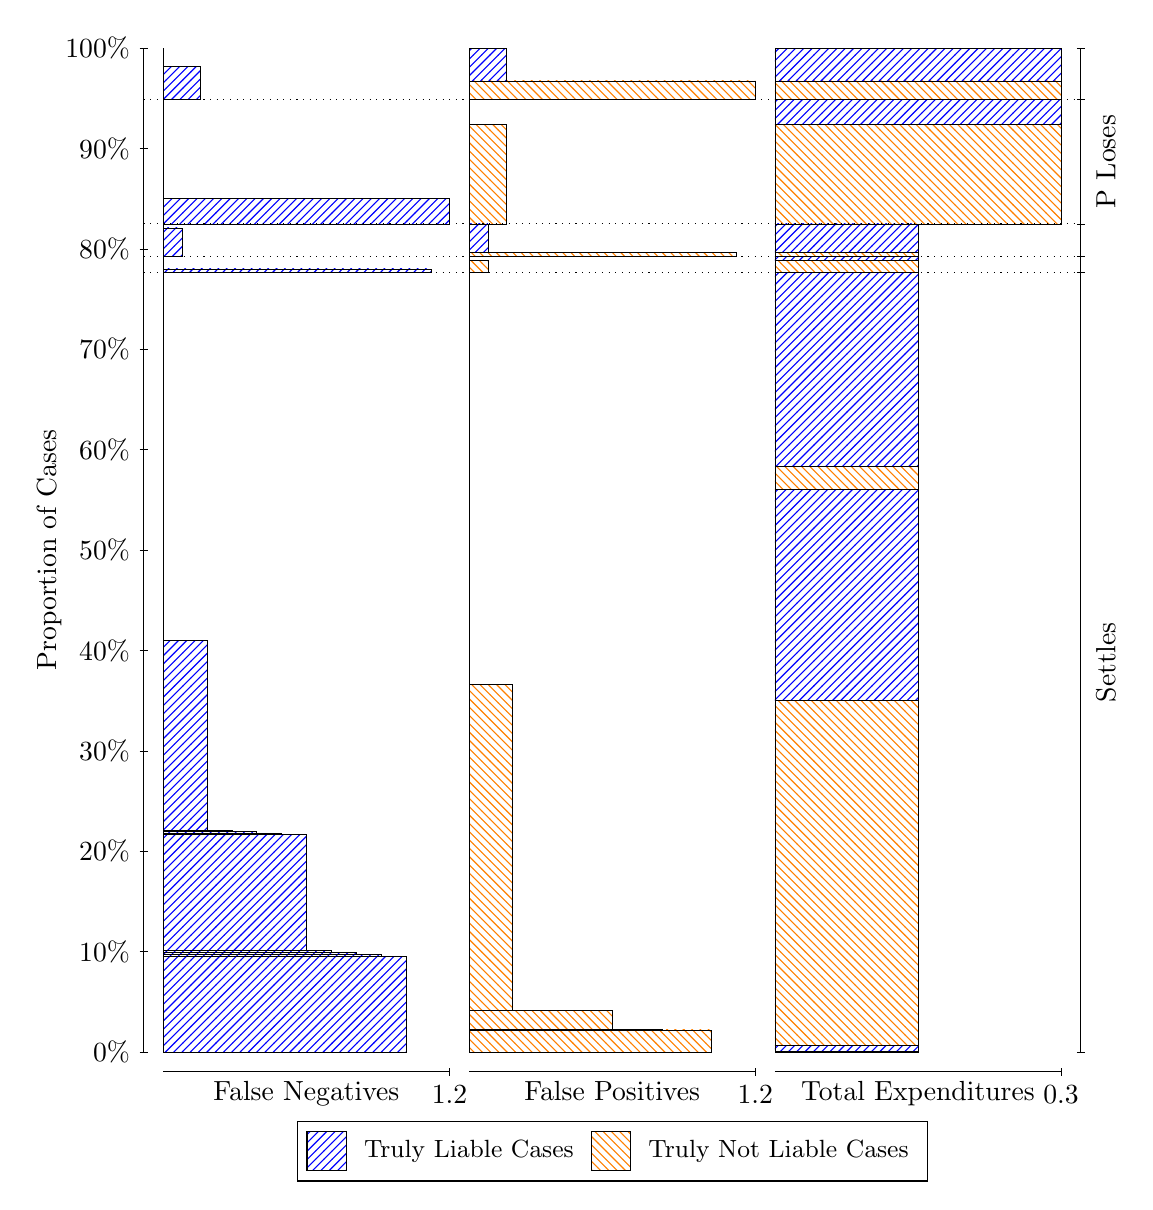
\begin{tikzpicture}
\draw[black, very thin] (1.5,1.75) -- (1.5,14.5);
\node[rotate=90, anchor=center] at (0.3, 8.125) {Proportion of Cases};
\draw[black, very thin] (1.45,1.75) -- (1.55,1.75);
\node[anchor=east] at (1.45, 1.75) {0\%};
\draw[black, very thin] (1.45,3.025) -- (1.55,3.025);
\node[anchor=east] at (1.45, 3.025) {10\%};
\draw[black, very thin] (1.45,4.3) -- (1.55,4.3);
\node[anchor=east] at (1.45, 4.3) {20\%};
\draw[black, very thin] (1.45,5.575) -- (1.55,5.575);
\node[anchor=east] at (1.45, 5.575) {30\%};
\draw[black, very thin] (1.45,6.85) -- (1.55,6.85);
\node[anchor=east] at (1.45, 6.85) {40\%};
\draw[black, very thin] (1.45,8.125) -- (1.55,8.125);
\node[anchor=east] at (1.45, 8.125) {50\%};
\draw[black, very thin] (1.45,9.4) -- (1.55,9.4);
\node[anchor=east] at (1.45, 9.4) {60\%};
\draw[black, very thin] (1.45,10.675) -- (1.55,10.675);
\node[anchor=east] at (1.45, 10.675) {70\%};
\draw[black, very thin] (1.45,11.95) -- (1.55,11.95);
\node[anchor=east] at (1.45, 11.95) {80\%};
\draw[black, very thin] (1.45,13.225) -- (1.55,13.225);
\node[anchor=east] at (1.45, 13.225) {90\%};
\draw[black, very thin] (1.45,14.5) -- (1.55,14.5);
\node[anchor=east] at (1.45, 14.5) {100\%};

\draw[black, very thin] (13.4,1.75) -- (13.4,14.5);
\draw[black, very thin] (13.35,1.75) -- (13.45,1.75);
\node[anchor=west] at (13.35, 1.75) {};
\draw[black, very thin] (13.35,11.648) -- (13.45,11.648);
\node[anchor=west] at (13.35, 11.648) {};
\draw[black, very thin] (13.35,11.852) -- (13.45,11.852);
\node[anchor=west] at (13.35, 11.852) {};
\draw[black, very thin] (13.35,12.268) -- (13.45,12.268);
\node[anchor=west] at (13.35, 12.268) {};
\draw[black, very thin] (13.35,13.849) -- (13.45,13.849);
\node[anchor=west] at (13.35, 13.849) {};
\draw[black, very thin] (13.35,14.5) -- (13.45,14.5);
\node[anchor=west] at (13.35, 14.5) {};

\draw[black, very thin, pattern color=blue, pattern=north east lines] (1.75,1.75) rectangle (4.8304,2.9631);
\draw[black, very thin, pattern color=blue, pattern=north east lines] (1.75,2.9631) rectangle (4.5145,2.9895);
\draw[black, very thin, pattern color=blue, pattern=north east lines] (1.75,2.9895) rectangle (4.1986,3.0169);
\draw[black, very thin, pattern color=blue, pattern=north east lines] (1.75,3.0169) rectangle (3.8826,3.0448);
\draw[black, very thin, pattern color=blue, pattern=north east lines] (1.75,3.0448) rectangle (3.5667,4.5128);
\draw[black, very thin, pattern color=blue, pattern=north east lines] (1.75,4.5128) rectangle (3.2507,4.5308);
\draw[black, very thin, pattern color=blue, pattern=north east lines] (1.75,4.5308) rectangle (2.9348,4.5489);
\draw[black, very thin, pattern color=blue, pattern=north east lines] (1.75,4.5489) rectangle (2.6188,4.5667);
\draw[black, very thin, pattern color=blue, pattern=north east lines] (1.75,4.5667) rectangle (2.3029,6.9748);
\draw[black, very thin, pattern color=orange, pattern=north west lines] (1.75,6.9748) rectangle (1.75,11.648);
\draw[black, very thin, pattern color=blue, pattern=north east lines] (1.75,11.648) rectangle (5.1464,11.696);
\draw[black, very thin, pattern color=orange, pattern=north west lines] (1.75,11.696) rectangle (1.75,11.852);
\draw[black, very thin, pattern color=blue, pattern=north east lines] (1.75,11.852) rectangle (1.987,12.215);
\draw[black, very thin, pattern color=orange, pattern=north west lines] (1.75,12.215) rectangle (1.75,12.268);
\draw[black, very thin, pattern color=blue, pattern=north east lines] (1.75,12.268) rectangle (5.3833,12.59);
\draw[black, very thin, pattern color=orange, pattern=north west lines] (1.75,12.59) rectangle (1.75,13.849);
\draw[black, very thin, pattern color=blue, pattern=north east lines] (1.75,13.849) rectangle (2.2239,14.266);
\draw[black, very thin, pattern color=orange, pattern=north west lines] (1.75,14.266) rectangle (1.75,14.5);
\draw[black, very thin, pattern color=orange, pattern=north west lines] (5.6333,1.75) rectangle (8.7138,2.0292);
\draw[black, very thin, pattern color=orange, pattern=north west lines] (5.6333,2.0292) rectangle (8.3978,2.0319);
\draw[black, very thin, pattern color=orange, pattern=north west lines] (5.6333,2.0319) rectangle (8.0819,2.0346);
\draw[black, very thin, pattern color=orange, pattern=north west lines] (5.6333,2.0346) rectangle (7.7659,2.0373);
\draw[black, very thin, pattern color=orange, pattern=north west lines] (5.6333,2.0373) rectangle (7.45,2.2756);
\draw[black, very thin, pattern color=orange, pattern=north west lines] (5.6333,2.2756) rectangle (7.1341,2.2756);
\draw[black, very thin, pattern color=orange, pattern=north west lines] (5.6333,2.2756) rectangle (7.1341,2.2775);
\draw[black, very thin, pattern color=orange, pattern=north west lines] (5.6333,2.2775) rectangle (6.8181,2.2794);
\draw[black, very thin, pattern color=orange, pattern=north west lines] (5.6333,2.2794) rectangle (6.5022,2.2812);
\draw[black, very thin, pattern color=orange, pattern=north west lines] (5.6333,2.2812) rectangle (6.1862,6.4228);
\draw[black, very thin, pattern color=blue, pattern=north east lines] (5.6333,6.4228) rectangle (5.6333,11.648);
\draw[black, very thin, pattern color=orange, pattern=north west lines] (5.6333,11.648) rectangle (5.8703,11.804);
\draw[black, very thin, pattern color=blue, pattern=north east lines] (5.6333,11.804) rectangle (5.6333,11.852);
\draw[black, very thin, pattern color=orange, pattern=north west lines] (5.6333,11.852) rectangle (9.0297,11.905);
\draw[black, very thin, pattern color=blue, pattern=north east lines] (5.6333,11.905) rectangle (5.8703,12.268);
\draw[black, very thin, pattern color=orange, pattern=north west lines] (5.6333,12.268) rectangle (6.1072,13.527);
\draw[black, very thin, pattern color=blue, pattern=north east lines] (5.6333,13.527) rectangle (5.6333,13.849);
\draw[black, very thin, pattern color=orange, pattern=north west lines] (5.6333,13.849) rectangle (9.2667,14.083);
\draw[black, very thin, pattern color=blue, pattern=north east lines] (5.6333,14.083) rectangle (6.1072,14.5);
\draw[black, very thin, pattern color=orange, pattern=north west lines] (9.5167,1.75) rectangle (11.333,1.7556);
\draw[black, very thin, pattern color=blue, pattern=north east lines] (9.5167,1.7556) rectangle (11.333,1.8373);
\draw[black, very thin, pattern color=orange, pattern=north west lines] (9.5167,1.8373) rectangle (11.333,6.2172);
\draw[black, very thin, pattern color=blue, pattern=north east lines] (9.5167,6.2172) rectangle (11.333,8.8984);
\draw[black, very thin, pattern color=orange, pattern=north west lines] (9.5167,8.8984) rectangle (11.333,9.1857);
\draw[black, very thin, pattern color=blue, pattern=north east lines] (9.5167,9.1857) rectangle (11.333,11.648);
\draw[black, very thin, pattern color=orange, pattern=north west lines] (9.5167,11.648) rectangle (11.333,11.804);
\draw[black, very thin, pattern color=blue, pattern=north east lines] (9.5167,11.804) rectangle (11.333,11.852);
\draw[black, very thin, pattern color=orange, pattern=north west lines] (9.5167,11.852) rectangle (11.333,11.905);
\draw[black, very thin, pattern color=blue, pattern=north east lines] (9.5167,11.905) rectangle (11.333,12.268);
\draw[black, very thin, pattern color=orange, pattern=north west lines] (9.5167,12.268) rectangle (13.15,13.527);
\draw[black, very thin, pattern color=blue, pattern=north east lines] (9.5167,13.527) rectangle (13.15,13.849);
\draw[black, very thin, pattern color=orange, pattern=north west lines] (9.5167,13.849) rectangle (13.15,14.083);
\draw[black, very thin, pattern color=blue, pattern=north east lines] (9.5167,14.083) rectangle (13.15,14.5);
\draw[black, dotted] (1.5,11.648) -- (13.4,11.648);
\draw[black, dotted] (1.5,11.852) -- (13.4,11.852);
\draw[black, dotted] (1.5,12.268) -- (13.4,12.268);
\draw[black, dotted] (1.5,13.849) -- (13.4,13.849);
\draw[black, very thin] (1.75,1.5) -- (5.3833,1.5);
\node[anchor=north] at (3.5667, 1.5) {False Negatives};
\draw[black, very thin] (5.3833,1.45) -- (5.3833,1.55);
\node[anchor=north] at (5.3833, 1.45) {1.2};

\draw[black, very thin] (5.6333,1.5) -- (9.2667,1.5);
\node[anchor=north] at (7.45, 1.5) {False Positives};
\draw[black, very thin] (9.2667,1.45) -- (9.2667,1.55);
\node[anchor=north] at (9.2667, 1.45) {1.2};

\draw[black, very thin] (9.5167,1.5) -- (13.15,1.5);
\node[anchor=north] at (11.333, 1.5) {Total Expenditures};
\draw[black, very thin] (13.15,1.45) -- (13.15,1.55);
\node[anchor=north] at (13.15, 1.45) {0.3};

\node[black, centered, rotate=90] at (13.72, 6.6988) {Settles};


\node[black, centered, rotate=90] at (13.72, 13.058) {P Loses};


\draw (7.449999999999999,1.5) node[draw=none] (baseCoordinate) {};
\begin{scope}[align=center]
        \matrix[scale=0.5, draw=black, below=0.5cm of baseCoordinate, nodes={draw}, column sep=0.1cm]{
            \node[rectangle, draw, minimum width=0.5cm, minimum height=0.5cm, pattern=north east lines, pattern color=blue] {}; &
            \node[draw=none, font=\small] (B) {Truly Liable Cases}; &
            \node[rectangle, draw, minimum width=0.5cm, minimum height=0.5cm, pattern=north west lines, pattern color=orange] {}; &
            \node[draw=none, font=\small] (B) {Truly Not Liable Cases}; \\
            };
\end{scope}

\end{tikzpicture}
\end{document}